\documentclass[conference]{IEEEtran}
\usepackage{graphicx}
\graphicspath{{./gambar/}}

\title{Analisis kekuatan Sinyal}

\author{Andrian Syah\IEEEauthorrefmark{1}, Hani Khairiyah\IEEEauthorrefmark{2}\\
\textit{Fakultas Teknologi Informasi}\\
\textit{Teknik Komputer}\\
\textit{Institut Teknologi Batam}\\
Batam, Indonesia\\
Email: \{\IEEEauthorrefmark{1}1922009, \IEEEauthorrefmark{2}1922001\}@student.iteba.ac.id}


\begin{document}
\maketitle

\begin{abstract}
    Implementasi jaringan wireless Atau yang biasa disebut dengan teknologi WLAN(Wireless Local Area Network) yang telah diatur oleh standar
    IEEE 802.11 . Jaringan WiFi digunakan untuk menghubungkan berbagai perangkat dan berbagi data.
    Analisis Wireless atau jaringan nirkabel menggunakan aplikasi InSSIDer ,
    Mengumpulkan Informasi jaringan yang ada pada sekitar lingkungan yang memiliki transmisi sinyal WiFi
\end{abstract}

\begin{IEEEkeywords}
    IEEE 802.11,InSSIDer,Wireless
\end{IEEEkeywords}

\section{Introduction}
Seiring berkembang nya zaman Teknologi semakin tidak bisa dihindarkan, 
kita sebagai manusia tidak dapat menghindar dari adanya teknologi tersebut,
banyak nya teknologi membuat banyak hal berubah sehingga menjadikan teknologi tersebut 
adalah bagian dari hidup. salah satu dari teknologi tersebut adalah teknologi jaringan nirkabel atau bisa disebut teknologi jaringan Wireless , yang dimana banyak digunakan di berbagai macam tempat  contoh nya dikampus,kafe,kedai kopi, dan lain-lain .

perkembangan Wireless ini sangat pesat sekali,karena flexible tanpa menggunakan kabel dan menghemat biaya 
, namun dari pernyataan tersebut Wireless juga banyak kelebihan dan kekurangan nya . 
Sebelumnya dianggap bahwa jaringan kabel lebih cepat dan lebih aman daripada jaringan nirkabel.
Namun peningkatan berkelanjutan pada teknologi jaringan nirkabel seperti standar jaringan Wireless
 telah membuat banyak perbedaan kecepatan dan keamanan antara jaringan kabel dan nirkabel tersebut.

 \begin{itemize}
    \item Local Area Network
\end{itemize}

Jaringan area lokal (LAN) dirancang untuk menghubungkan komputer pribadi dan perangkat digital lainnya dalam radius setengah mil atau 500 meter. 
LAN biasanya menghubungkan beberapa komputer di kantor kecil, semua komputer di satu gedung, atau semua komputer di beberapa gedung dalam jarak dekat.
Sistem operasi LAN yang paling umum adalah Windows, Linux, dan lain-lain

\begin{itemize}
    \item Wide Area Networks (WAN)
\end{itemize}
Wide area networks (WAN) menjangkau jarak geografis yang luas (seluruh wilayah, negara bagian, benua, atau seluruh dunia). 
WAN yang paling universal dan kuat adalah Internet.
Komputer terhubung ke WAN melalui jaringan publik, seperti sistem telepon atau sistem kabel pribadi, atau melalui leased line atau satelit. 
Jaringan area metropolitan (MAN) adalah jaringan yang mencakup area metropolitan, biasanya kota dan pinggiran kota utamanya. 
Lingkup geografisnya berada di antara WAN dan LAN.

\begin{itemize}
    \item Metropolitan Area Network (MAN)
\end{itemize}
MAN atau Metropolitan Area Network mencakup area yang lebih besar daripada LAN dan area yang lebih kecil dibandingkan dengan WAN.
Ini menghubungkan dua atau lebih komputer yang terpisah tetapi berada di kota yang sama atau berbeda. 
Ini mencakup area geografis yang luas dan dapat berfungsi sebagai ISP (penyedia layanan internet).
MAN dirancang untuk pelanggan yang membutuhkan konektivitas berkecepatan tinggi.
Kecepatan MAN berkisar dalam hal Mbps. Sulit untuk merancang dan memelihara Jaringan Area Metropolitan. 
Toleransi kesalahan dari MAN lebih sedikit daripada LAN dan juga ada lebih banyak kemacetan di jaringan.
Kecepatan transfer data dan penundaan propagasi dari MAN adalah moderat.

\begin{itemize}
    \item Personal Area Network (PAN)
\end{itemize}
Mewakili teknologi personal area network wireless seperti Bluetooth (IEEE 802.15) dan Infrared (IR). 
Jaringan ini mengizinkan hubungan peralatan personal dalam suatu area berkisar 12 inchi. 
Bagaimanapun juga Infrared membutuhkan hubungan langsung dan jangkauan yang lebih pendek.

\section{Related Work}
Wi-Fi atau lebih dikenal dengan
WLAN (Wireless Local Area Network) merupakan
teknologi jaringan wireless yang ditujukan untuk
menghubungkan beberapa terminal berbasis IP (PC,
notebook atau PDA) dalam suatu area LAN (Local
Area Network). WLAN merupakan salah satu apli-
kasi pengembangan wireless untuk komunikasi data.
Sesuai dengan namanya yaitu wireless, berarti tanpa
kabel, WLAN adalah jaringan lokal yang tidak me-
nggunakan kabel . Jaringan WLAN
sangat efektif digunakan didalam sebuah kawasan
atau gedung. Dengan performa dan keamanan yang
dapat diandalkan, pengembangan jaringan WLAN
menjadi tren baru pengembangan jaringan meng-
gantikan jaringan wired atau jaringan penuh kabel.
Solusi dari pengembangan WLAN dapat mencakup
sebuah kawasan rumah, kantor kecil, perusahaan
hingga ke area-area publik~. 

Menurut Andi Maslan dan Tonny Wangdra, Wi-Fi adalah
satu standar wireless networking, hanya dengan komponen yang sesuai dapat
terkoneksi ke jaringan (2012 :105). Menurutnya, teknologi Wi-Fi memiliki standar
protocol yang ditetapkan oleh sebuah institut internasional yang bernama Institute of
Electrical and Electronic Engineers (IEEE), yang secara umum sebagai berikut : 

\begin{itemize}
    \item Standar IEEE 802.11a yaitu Wi-Fi dengan frekuensi 5 GHz yang memiliki
    kecepatan 54 Mbps dan jangkauan jaringan 300m. 
    \item Standar IEEE 802.11b yaitu Wi-Fi dengan frekuensi 2.4 GHz yang memiliki
    kecepatan 11 Mbps dan jangkauan jaringan 100m. 
    \item Standar IEEE 802.11g yaitu Wi-Fi dengan frekuensi 2.4 GHz yang memiliki
    kecepatan 54 Mbps dan jangkauan jaringan 300m.
\end{itemize}

\begin{table}[htbp]
    \caption{Table Specification Wifi and Compability}
    \begin{center}
    \begin{tabular}{|c|c|c|c|}
        \hline
    \textbf{Specification} & \textbf{\textit{speed}}& \textbf{\textit{frequency band}}& \textbf{\textit{Series Compability}} \\
    \hline
    802.11b & 11Mb/s & 2.4GHz & b  \\
    \hline
    802.11a & 54Mb/s & 5GHz & a  \\
    \hline
    802.11g & 54Mb/s & 2.4GHz & b,g  \\
    \hline
    802.11n & 100Mb/s & 2.4GHz & b,g,a  \\
    \hline
    \multicolumn{4}{l}{$^{\mathrm{a}}$Wahana Komputer,2010}
    \end{tabular}
    \label{tab1}
    \end{center}
    \end{table}


\subsection{Pengukuran RSSI (Receive Signal Strength indicator)}
RSSI adalah sebuah teknologi yang sering digunakan untuk mengukur suatu indikator kekuatan transimisi
data / sinyal yang diterima oleh receiver suatu perangkat wireless . biasa nya RSSI digunakan untuk memetakn
nilai berdasarkan jarak,ketinggan,penghalang, dan lain-lain . 

Daya yang diterima oleh antenna (Pr) ditempatkan pada jarak d
dari antenna pemancar dengan jumlah yang diketahui
ditansmisikan daya (Pt) dan diberikan oleh
persamaan Friis pada persamaan :

\begin{equation}
    Pr = P_t G_r G_t 
    \left( 
        \frac{\lambda}{4 \pi d}
    \right) ^2
\end{equation}

dimana Gt merupakan Gain dari antena pemancar, Gr
adalah Gain dari antena penerima  dan lambda adalah
panjang gelombang~. \cite{puspitasari2014analisis}

disini pengaruh suhu dan kekuatan angin sangat berpengaruh terhadap kualitas RSSI ,
untuk diruangan dan didalam ruangan akan terdapat perbedaan yang sangat signifikan , faktor-faktor
yang mempengaruhi transmisi sinyal pada suatu receiver adalah hambatan seperti dinding,ketinggan , kualitas transmiter , dan lain-lain .
kinerja pada sinyal yang menggunakan band 2,4 Ghz pada suatu waktu akan terjadi noise apabila yang digunakan pada device adalah NIC yang abal-abal. 

\subsection{Pengaruh Berbagai Faktor pada RSSI dari Positioning Antena}
Pengaruh faktor pada RSSI terhadap Positioning dari antena pada Usb wireless TL-WN722N \cite{LINK2018} sangat bengaruh terhadap penerimaaan data yang ada pada device / Laptop
hal ini memungkinkan terjadi nya transmisi yang tidak stabil apabila menggunakan aplikasi InSSIDer dan digunakan SpeedTest untuk mengetest kecepatan transfer data .

\section{Scenario}
Pada sesi ini kami menggunakan skenario menggunakan peralatan seperti dibawah ini :
\subsection{Alat dan Bahan}

\begin{itemize}
    \item Access Point : akses point yang digunakan pada sesi ini adalah akses point dengan SSID  "Alfatih" , dengan menggunakan vendor router Huawei HG8245 dengan transimisi 100\% 
    \item Laptop : Laptop yang digunakan adalah merk HP dengan series 8440p dengan sistem operasi windows dual boot ubuntu , processor i5 generasi 1 ,dengan penyimpanan 1 TB ,dan RAM sebesar 6 GB 
    \item Handphone : Redmi Note 8 dengan RAM 4 GB dan penyimpanan internal sebesar 64 GB 
    \item USB Wireless : TP-LINK TL-WN722N dengan kecepatan maksimal transfer data sebesar 150 Mbps ~
    \item Meteran : untuk mengukur jarak router ke receiver
\end{itemize}

\subsection{Software yang digunakan}

\begin{itemize}
    \item Aplikasi InSSIDer :berfungsi sebagai scanner WiFi yang dapat dijangkau oleh adapter WiFi dengan hasil yang sangat terperinci dari setiap masing-masing jaringan WiFi. Kelebihan lain dari software inSSIDer ini ialah dapat bekerja pada merek adapter WiFi biasa jadi tidak membutuhkan adapter / perangkat WiFi yang khusus.
    \item Speedtest by Ookla : sebuah situs yang menyediakan pengujian kecepatan koneksi internet yang disediakan oleh perusahaan asal Kalispel .
\end{itemize}

\subsection{Teknik Pengumpulan Data}

\begin{itemize}
    \item Melakukan perencanaan penelitian yang membahas mengenai data yang akan diambil
pada saat penelitian meliputi denah, tinggi
access point, koordinat, jarak, RSSI 

    \item Menentukan koordinat posisi Access Point
dan posisi receiver di lingkungan indoor.

    \item Aplikasi inSSIDER yang telah dijalankan
akan melaporkan data terhadap nilai RSSI
yang diterima oleh receiver, dan
pengumpulan data selesai
\end{itemize}

Pengukuran yang dilakukan terhadap sinyal transmisi ini seperti dibawah ini :

\begin{figure}[h]
    \centering
    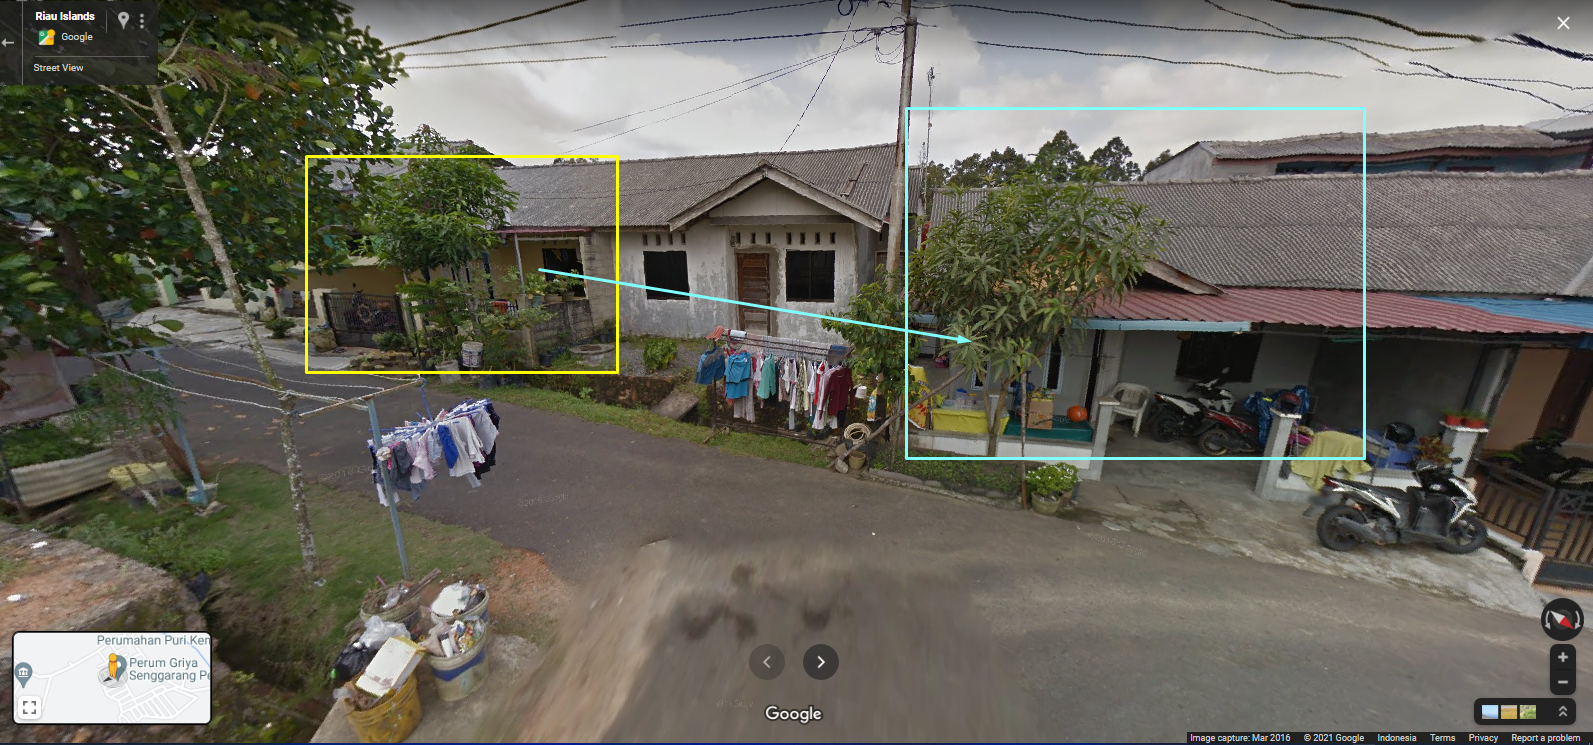
\includegraphics[width=0.5\textwidth]{gambar-lokasi.png}
    \caption{Denah Lokasi Pengukuran Jarak}
\end{figure}

pada gambar diatas diukur menggunakan meteran jarak nya adalah 8.5 Meter dengan posisi Router berada didalam rumah 
kondisi ini memiliki hambatan karena terdapat beberapa dinding yang harus ditembus sinyal . sehingga yang didapatkan pada receiver TL-WN722N tidak stabil .

\begin{figure}[h]
    \centering
    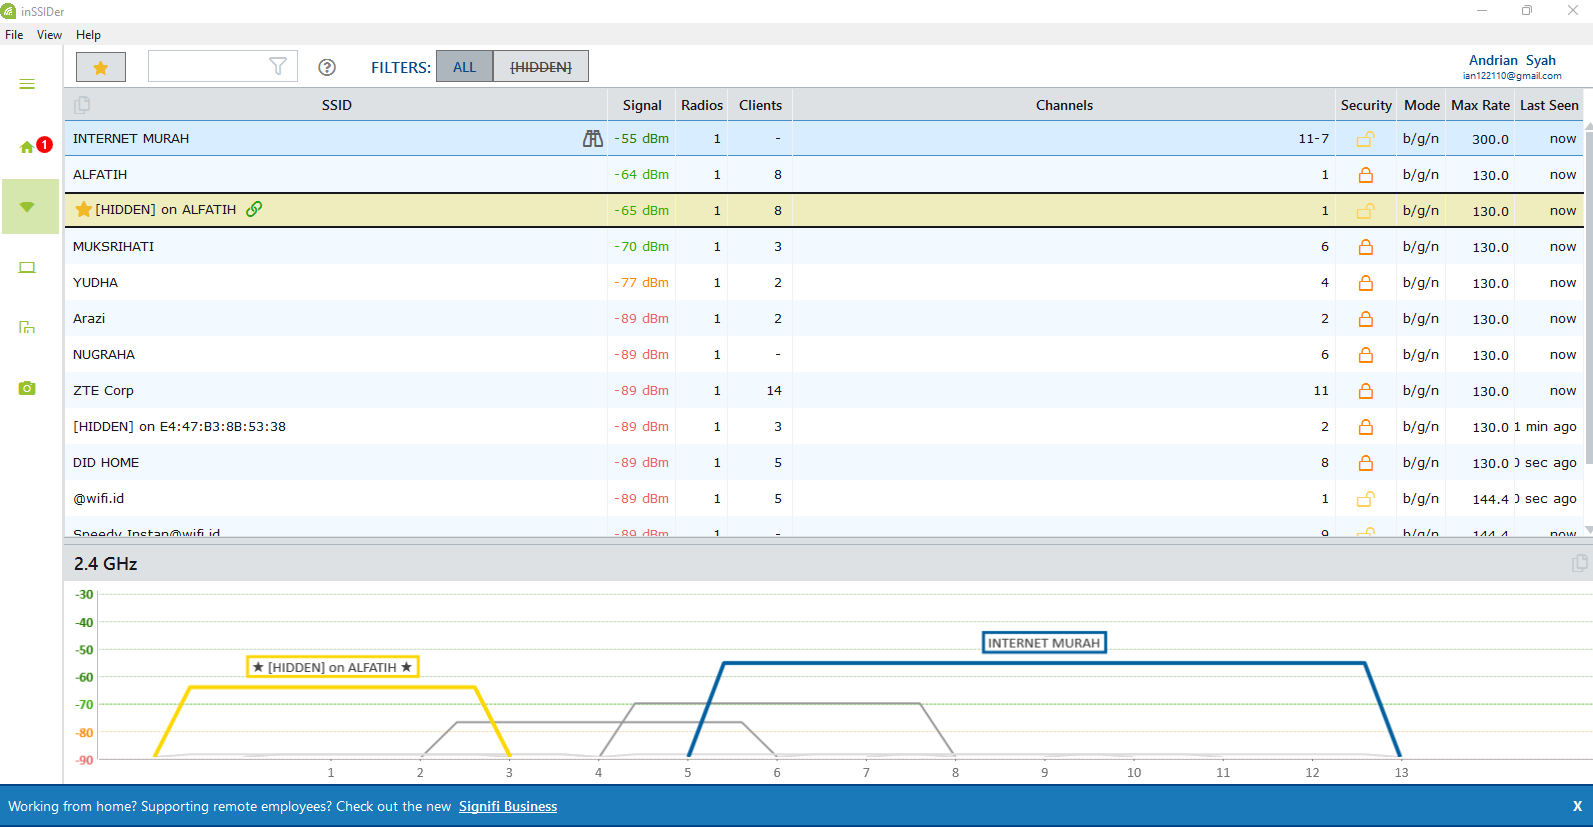
\includegraphics[width=0.5\textwidth]{gambar-inssider.png}
    \caption{Analisis InSSIDer}
\end{figure}

didapatkan sinyal yang bernama "ALFATIH" sebesar -65dBm dalam posisi HIDDEN , jika kita liat HIDDEN ini berarti terdapat SSID yang di enable kan untuk broadcast atau dipancarkan .

\begin{figure}[h]
    \centering
    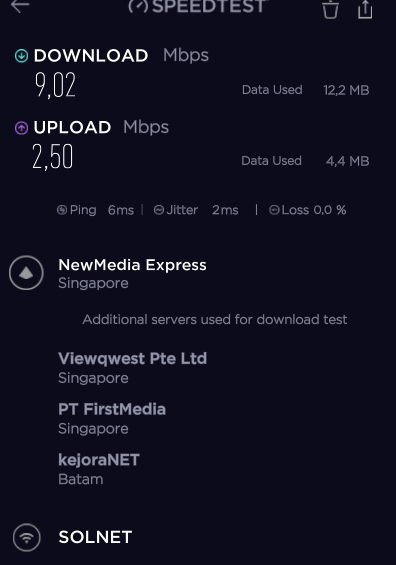
\includegraphics[width=0.4\textwidth]{speedtest.png}
    \caption{SpeedTest}
\end{figure}

pada pengetesan kali ini , hambatan yang ada antara receiver dan router adalah tembok yang hanya di sekat . dapat kita lihat bahwa kecepatan yang di dapatkan dari ISP Seharus nya 1:2 dengan paket 25 Mbps .

\begin{figure}[h]
    \centering
    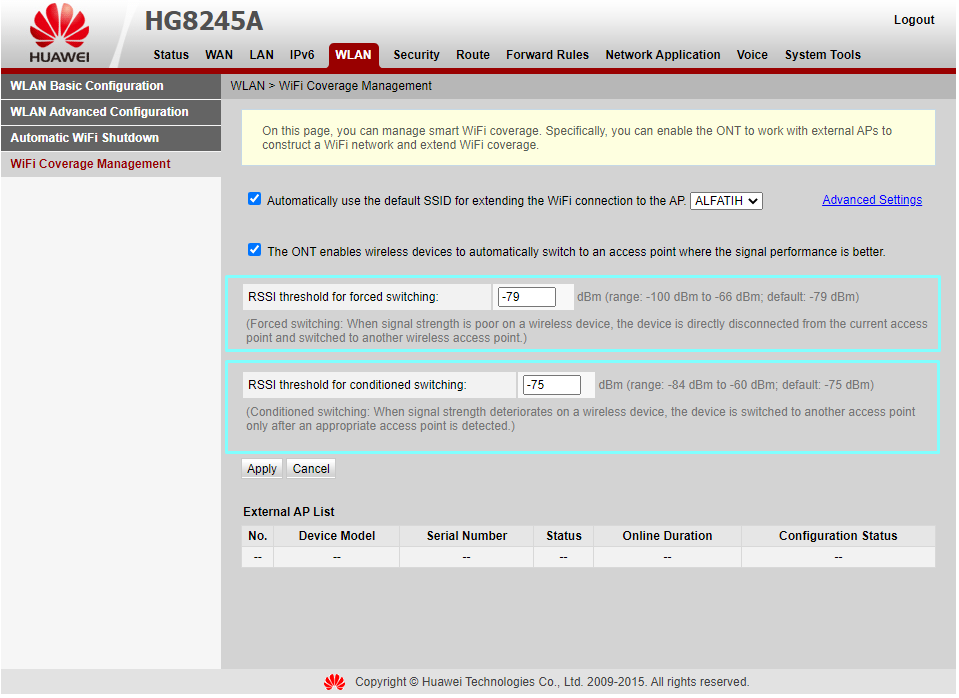
\includegraphics[width=0.5\textwidth]{router.png}
    \caption{Halaman Admin Pada Router Huawei}
\end{figure}


\begin{figure}[h]
    \centering
    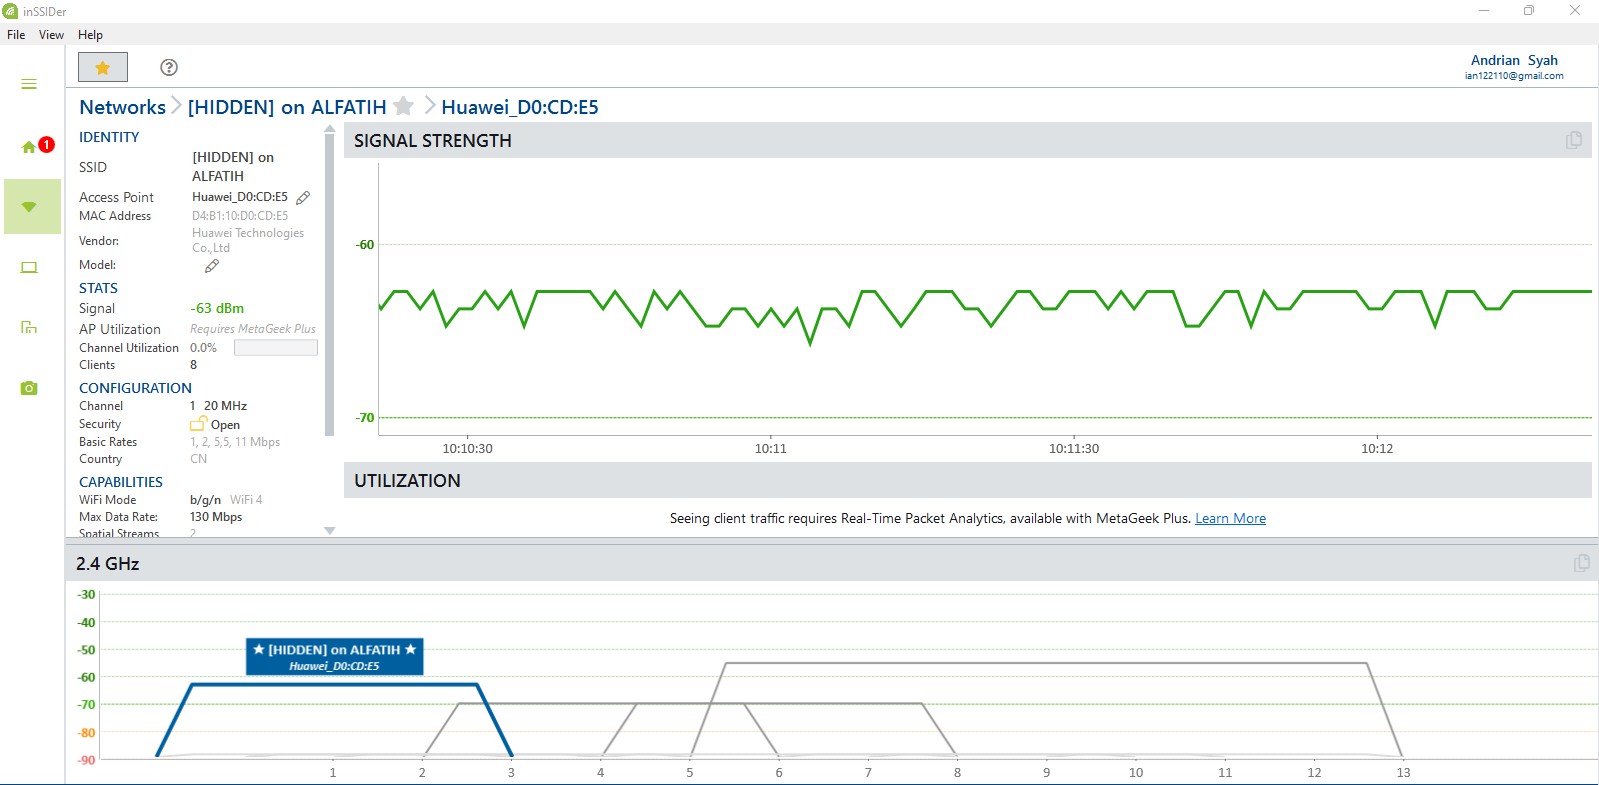
\includegraphics[width=0.5\textwidth]{signal-strengh.png}
    \caption{Halaman Admin Pada Router Huawei}
\end{figure}

Kekuatan sinyal RSSI yang diterima oleh
receiver tidak bergantung dengan  adanya jarak
antara transmitter dan receiver, akan tetapi
menunjukkan terdapat berbagai variasi yang besar terhadap fading
dan shadowing pada sebuah lokasi. Hal ini
terlihat pada tempat pengukuran yang kondisi
lingkungannya memiliki banyak property seperti
didalam ruangan terdapat sekat, tembok, meja dan 
property lainnya, sehingga akan terjadi peredaman sinyal, pembelokan sinyal dan pemantulan
sinyal yang mengakibatkan penurunan kuat
sinyal yang dipancarkan oleh transmiter kepada
receiver, walaupun jarak antara transmiter dan
receiver cukup dekat, namun terhalang oleh
adanya property disekitarnya, maka kekuatan
sinyalnya akan menurun dan kemungkinan
kekuatan sinyal nya akan sama dengan kekuatan
sinyal pada jarak antara transmiter dan receiver
yang cukup jauh, namun tidak memiliki
penghalang disekitarnya. 

\section{Hasil dan Pembahasan}

*under way

Dari hasi analisis jaringan wireless yang dilakukan pada lingkungan kampus
institut teknologi batam menggunakan alat usb wireless penerima sinyal TP-LINK TL-WN722N yaitu pada saat kami berjalan menuju lantai 2 di area kampus iteba , jaringan akan berpindah
ke akses point terdekat dengan SSID yang sama , karena penggunaaan repeater yang ada dikampus yang menyebabkan apabila terjadi permasalahan
pada pusat jaringan atau Router Utama maka akan terjadi lost koneksi pada setiap semua repeater yang ada .
disini kami juga mencoba kecepatan internet pada SSID Iteba Student menggunakan aplikasi SpeedTest By Ookla~\cite{Ookla}.

\begin{equation}
    Rerata RSSI = \frac{Total Jumlah Nilai RSSI}{Jumlah Koordinat receiver}
    \label{rerata_rssi}
\end{equation}

\begin{table}[htbp]
    \caption{Table Analisis Pengukuran RSSI}
    \begin{center}
    \begin{tabular}{|c|c|c|c|}
        \hline
    \textbf{Nomor} & \textbf{\textit{Tinggi}}& \textbf{\textit{Receiver}}& \textbf{\textit{Rata-rata sinyal penerima}} \\
    \hline
    1 & 150cm& 25 Receiver & -53.87 dbm  \\
    \hline
    2 & 200cm& 15 Receiver & -51.98 dbm  \\
    \hline
    \multicolumn{4}{l}{$^{\mathrm{a}}$Hasil dari dana InSSIDer}
    \end{tabular}
    \label{tab2}
    \end{center}
    \end{table}

\section{Kesimpulan}
Dapat disimpulkan bahwa saat pengetesan menggunakan aplikasi InSSIDer kekuatan sinyal juga mempengaruhi transmisi data yang dimana ini menggunakan internet,
sehingga ada nya perbedaan pada saat ada nya penghalang sewaktu pengetesan dan tidak adanya penghalang saat pengetesan , beberapa keunggulan dan kekurangan dari wireless network 
sangat mungkin ada , karena pada dasarnya manusia menciptakan sesuatu hal yang belum sempurna namun dari pernyataan tersebut bahwa manusia membuat perangkat nirkabel untuk memudahkan pengaksesan 
tanpa menggunakan perantara kabel saat terkoneksi di device , perangkat hardware pada device juga mempengaruhi kekuatan sinyal , karena apabila hardware penangkap sinyal yang ada pada suatu komputer sudah usang atau sudah rusak , maka sinyal transmisi yang dihasilkan akan lebih jauh menurun.

\bibliographystyle{IEEEtran}
\bibliography{referensi.bib}

\end{document}